\documentclass[tikz, preview]{standalone}
\usepackage{amsfonts, amsthm, amssymb, amsmath, stmaryrd, etoolbox}
\usepackage{tikz}
\usetikzlibrary{matrix,arrows}
\tikzset{->-/.style={decoration={markings, mark=at position .5 with {\arrow{>}}},postaction={decorate}}}
\tikzset{->-pos/.style={decoration={markings, mark=at position #1 with {\arrow{>}}},postaction={decorate}}}
\tikzset{->-/.style={decoration={markings,mark=at position .5 with {\arrow{>}}},postaction={decorate}}}
\tikzset{->-pos/.style={decoration={markings,mark=at position #1 with {\arrow{>}}},postaction={decorate}}}

\begin{document}
%%%%%%%%%%%%%%%%% 
%%%%%%%%%%%%%%%%% 
\[
  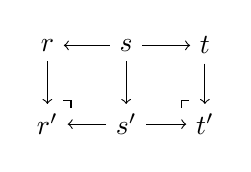
\begin{tikzpicture}
    %draw [help lines, step=0.2, color=blue!10] (-5,-5) grid (5,5); % grid
    % 
    \node (1) at (-1,1) {$ r $};
    \node (2) at (-1,0) {$ r' $};
    \node (3) at (0,1) {$ s $};
    \node (4) at (0,0) {$ s' $};
    \node (5) at (1,1) {$ t $};
    \node (6) at (1,0) {$ t' $};
    %
    \draw [->] (3) to node [] {$  $} (1);
    \draw [->] (3) to node [] {$  $} (5);
    \draw [->] (4) to node [] {$  $} (2);
    \draw [->] (4) to node [] {$  $} (6);
    \draw [->] (1) to node [] {$  $} (2);
    \draw [->] (3) to node [] {$  $} (4);
    \draw [->] (5) to node [] {$  $} (6);
    %
    \draw (-0.8,0.3) -- (-0.7,0.3) -- (-0.7,0.2);
    \draw (0.8,0.3) -- (0.7,0.3) -- (0.7,0.2);
  \end{tikzpicture}
\]
%%%%%%%%%%%%%%%%% 
%%%%%%%%%%%%%%%%% 
\end{document}
